\documentclass[10pt,a4paper]{article}
\usepackage[utf8]{inputenc}
\usepackage[scale=0.7,vmarginratio={1:2},heightrounded]{geometry}

\usepackage{multicol}
\setlength{\columnsep}{1cm}
\usepackage{scrextend}
\addtokomafont{labelinglabel}{\sffamily}
\usepackage[numbers]{natbib}

\usepackage[strings]{underscore}

% link support in pdf
\usepackage[colorlinks,allcolors=blue,breaklinks = true]{hyperref}

% images in pdf
\usepackage{graphicx}
\graphicspath{{Images/}}
% multiple images
\usepackage{subfigure}
% images float in text
\usepackage{float}

% url support
\usepackage{url}
% glossarie support
\usepackage[acronym, automake]{glossaries}
\makeglossaries
\loadglsentries{myGlossary}

% math libs
\usepackage{amsmath}
\usepackage{amssymb}
\usepackage{amstext}
\usepackage{amsfonts}
\usepackage{mathrsfs}

% Code formating
\usepackage{listings}
\usepackage{color}

% subfile to include titlepage. Possible to gitignore titlepage with private information
\usepackage{subfiles}

\definecolor{dkgreen}{rgb}{0,0.6,0}
\definecolor{gray}{rgb}{0.5,0.5,0.5}
\definecolor{mauve}{rgb}{0.58,0,0.82}

\lstset{frame=tb,
  language=Java,
  aboveskip=3mm,
  belowskip=3mm,
  showstringspaces=false,
  columns=flexible,
  basicstyle={\small\ttfamily},
  numbers=none,
  numberstyle=\tiny\color{gray},
  keywordstyle=\color{blue},
  commentstyle=\color{dkgreen},
  stringstyle=\color{mauve},
  breaklines=true,
  breakatwhitespace=true,
  tabsize=3
}

%Metadata
\title{TBD}
\author{Simon Hischier}
\date{April 2018}

\begin{document}

\subfile{titlepage}


%Table of Contents Page
\renewcommand{\contentsname}{Inhalt}
\tableofcontents
\newpage

%First real page
\section{Abstract}
\label{sec:abstract}
\begin{multicols}{2}
This work discusses the relation between the past lack of procedural content generation in the game industry with the recent uptake of procedural content generation in emerging tools for game developers and artists and the use of procedural content generation in the game industry. How is procedural content generation as part of games and as a developing tool changing so that it is gaining relevance in the games industry and related sectors? New tools and a more data-driven approach to procedural content generation in recent years has lead to a less noticeable but steady increase in usage across a number of disciplines and workfields and a shift in toolsets in the game industry. The paper observes and analyzes the trends and tries to explain the newfound interest through analogy, literature review, market and workflow analysis. We want to highlight what these new tools and approaches provide and what previous tools were missing and the conclusion why procedural content generation gains popularity again based on these changes.
\end{multicols}

\section{Introduction}
\begin{multicols}{2}
The cost to make games seems to be on an exponential curve as Raph Koster states\cite{Koster2018}. He suggests among other things that game developers should focus a lot more on algorithmic and procedural approaches to keep the cost of games under control. On Quora, an online discussion forum, Steve Theodore gives an example on the time needed for assets in games. A model for the game Half-Life 1 took about 2 working weeks and a model 10 years later took him seven working weeks. Theodore states, that most extra time is spent on texturing, shading and animation\cite{Prinke2017}. Those are fields where \gls{pcg} has seen huge improvements.

Studios developing AAA games spend a lot more money on creating resources. Samuel Rantaeskola\cite{Prinke2017} states that in the past systems were less powerful and therefore the limiting factor was optimization. Nowadays the content and increasing complexity of content is the big limitation. More people working on a project increases overhead and the more work on a project the less impact there is when a single person is added to a team.

Ever-increasing cost of development does come with side effects. A lot of big studios closed down or had massive layoffs over the past year \cite{Lahti2018, Schreier2019, Walker2019, Schreier2019a} and this seems to be a long term trend backed by older numbers\cite{Plunkett2012}. The race to higher costs leave midsize studios in an awkward position. They are too big to survive by creating small games but not big enough to compete with AAA games. Steve Theodore recalls seeing a lot of midsize studios closing down in the seattle area because they grew into big studios, went indie or died\cite{Prinke2017}.
\end{multicols}

\section{Problem/Research Question}
\begin{multicols}{2}
todo
\end{multicols}

\section{Literature Review}
\subsection{Categories of Procedural Generation}
We are using \gls{pcg} categories based on the book “Procedural Generation in Game Design”\citep[p.~3]{Short:2017:PGG:3161477} where the following four categories are described.

\begin{labeling}{categories}
\item [Integral] The use of \gls{pcg} is part of the game design from the start. This games rely heavily on a working PCG and even core gameplay can be affected. Games such as \textit{Rogue} (A.I. Design, 1980) or a more modern game like \textit{Dwarf Fortress} (Dwarf Fortress, 2006) are using \gls{pcg} extensively and would not work without it. They need it to be the type of game they are. Changes to the project planning have vast implications on the codebase. These games are build around central algorithms and project changes will result in redrafting the algorithms.

\item [Drafting Content] From a game design perspective this games do not rely on \gls{pcg} from the start. Game designers rely on PCG to generate initial drafts of game content such as the map or items. These drafts can be looked through by humans and are then handpicked. Some games use this method to generate a world which is then polished by humans. An example of generating and polishing is \textit{Skyrim} (Bethesda Game Studios, 2011) and a more recent and sophisticated example is \textit{Far Cry 5} (Ubisoft, 2018) where Carrier Étienne explains how the world was modified by humans but regenerated daily by his team\cite{Carrier2018}.

\item [Modal] Some games are build with little or even without the use for \gls{pcg} and it gets added later on during development. Even after release PCG can be added in the form of an “infinity mode” or as procedural maps in \textit{Rust} (Facepunch Studios Ltd, 2013). While this type can add a lot or replay value to a game it is mostly used just for that and does not add innovative content to the game.

\item [Segmented] A game build with segmented content including closed off areas where \gls{pcg} is used. The development can continue with or without these areas if the desired standard is not met by the algorithm. The term “areas” doesn’t need to be restricted to levels. It can include parts of the game such as procedural music, graphical effects or randomized elements. The game developers have at all times the possibility to revert to hand-generated content.
\end{labeling}

\subsection{Rise of Scripting languages}
\begin{multicols}{2}
John K. Ousterhout wrote a paper\cite{Ousterhout1998} in 1998 where he analyzed the difference in use of system languages (C, C++, Java) and scripting languages (Python, Perl, Javascript). His analysis is important because in this paper we look at visual node systems (a part of the dataflow programming paradigm\cite{wiki:Dataflow}) as comparable to scripting languages in the sense that they are more easily understandable. He pointed out, that scripting languages are much better suited for casual programmers based on several reasons.One reason is the size of programs. Scripting languages need less lines of code to get things done. Higher-level languages need several months of learning to master where as scripting languages lead to results in hours. This is of great importance, it allows a team to hire technical artists who are quickly ready to work on projects. However both languages are required, they are complementary.\begin{quote}
“Scripting languages assume that a collection of useful components already exists in other languages.”\citep[p.~2]{Ousterhout1998}
\end{quote}
The limiting factor in larger adaptations are the power of computers. The paper finds that, the faster computers get the larger the applications built with scripting languages will be. Current developments on various applications indicate that computers are powerful enough. Workflows are shifting towards programs with scripting languages or visual node systems.
\end{multicols}


\section{Methodology and Results}
\subsection{Textures}
\begin{multicols}{2}
Textures is traditionally a big topic in game development. A lot of research went into textures because it’s a big part of modern rendering pipelines and reaches back to the early days of modern computer graphics. Games in the 80’s and 90’s had hard limits on disk space\cite{Ferrari2016} and designing games involved balancing storage space between program code, music and images. As an example on the limitation: Besides a single digital sample channel sounds on home consoles like the \gls{nes} were limited to hardware generated tones\cite{wiki:NintendoEntertainmentSystem}. Consoles like the \gls{nes} and \gls{snes} had no chips to calculate complex 3D objects. The Picture Processing unit was used to display only sprites. To fill a TV screen the \gls{nes} and \gls{snes} used texture tiling, a technique for creating small texture samples which can be tiled to create a seamless pattern. This technique is still in use for modern games with increased more complex textures and increased texture size. Games using \gls{pcg} as an integral part rely heavily on tileable textures or alternatively use generated procedural textures for example Perlin\cite{perlin1985image} or Worley\cite{worley1996cellular} noise. Those approaches come with disadvantages: Tiles are very repetitive and Perlin noise need very sophisticated algorithms to generate interesting levels. Another texture generating solution is using by-example noise algorithms. These algorithms take a stochastic example texture and generate larger versions out of it. Until now these were too slow for real time generation and therefore were only suitable for drafting content. A recent paper by Heitz and Neyret created an algorithm able to create stochastic textures on-the-fly\cite{Heitz2018}. This enables artists to build levels and getting direct feedback with final textures already applied during building. This technique even allows for algorithmic level generation while not using tile based textures. This is especially important because textures not based on tiles lead to hard edges and repeating patterns shown in \autoref{fig:procStocTexturing}.
\end{multicols}

\begin{figure}[H]
    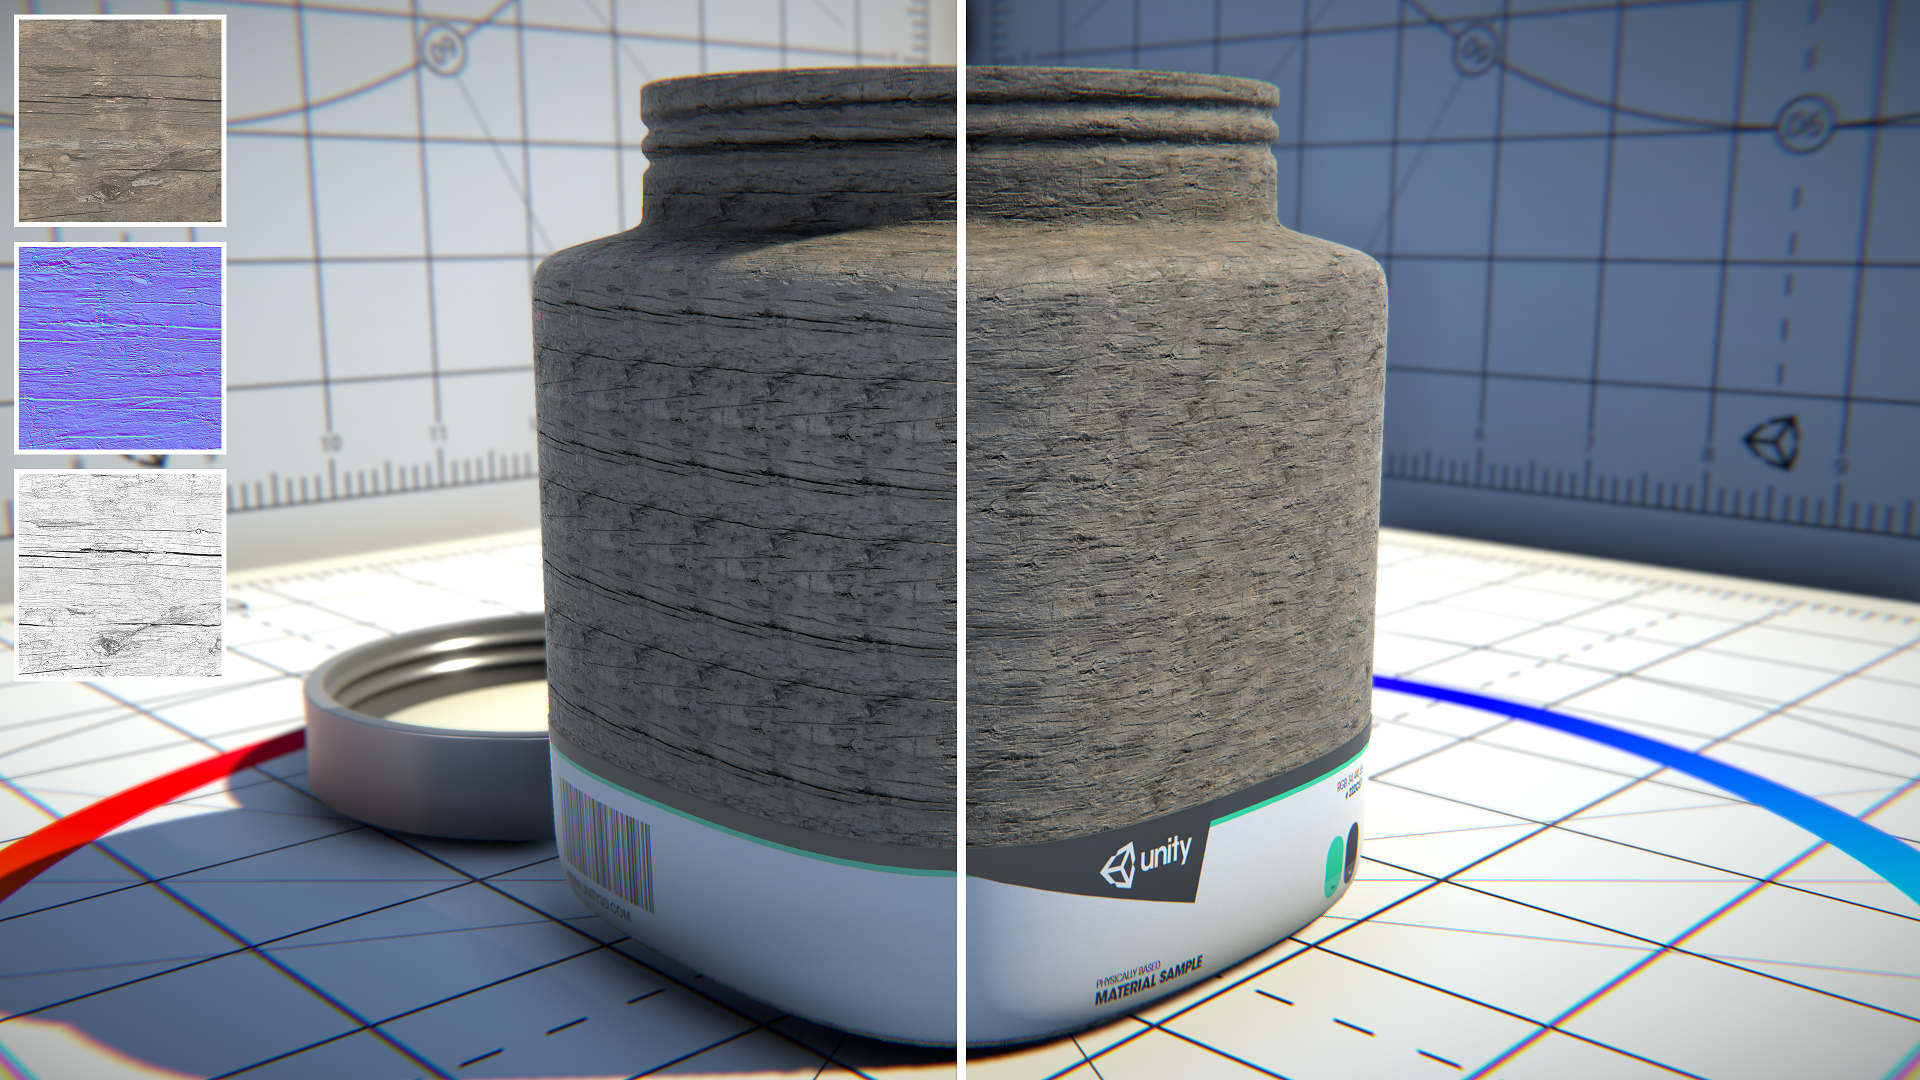
\includegraphics[width=\textwidth, height=\textheight, keepaspectratio]{proceduralStochasticTexturingInUnityExample.png}
    \caption{Wood detail maps with albedo, normal and occlusion textures. Retrieved 11:50, March 9, 2019 from {https://blogs.unity3d.com/2019/02/14/procedural-stochastic-texturing-in-unity/}}
    \label{fig:procStocTexturing}
\end{figure}

\subsection{Tools for Procedural Content Generation}
At the Blender Conference Andrew Price tried to predict changes to the 3D industry in the next 5 to 10 years. A big point besides machine learning assistance becoming a standard is the adaption of procedural workflows becoming mainstream\cite{Price2018}. Price states that procedural texturing made by Substance Designer in combination with Substance Painter is saving big studios money in the range of hundreds of thousands of US Dollars.

\section{Conclusion and Future Work}
\begin{multicols}{2}
todo
\end{multicols}



%
%\section{EXAMPLE TEXTS}
%from here on down are only examples
%\section{Abstract}
%\label{sec:abstractEx}
%We can Cite \cite{wikipediaScriptingLanguage}, \cite{Iivari2008usabilityInCompanyOSS}, \cite{almarzouq2005open}, \cite{heiseonline2017limuxservus}, \cite{viorres2007major}, \cite{wikipediaScriptingLanguage} etc. If we want to have terms and shortcuts we can introduce them once: \gls{longGlsEx} and \gls{oss}. If we refer to \gls{longGlsEx} and \gls{oss} later it will only use the short version.
%
%\section{Various examples}
%\subsection{crossreference}
%If we want to reference previous sections like (\hyperref[sec:abstractEx]{Abstract}) we can do that with a label and a reference. It is possible to automatically reference Sections \autoref{sec:abstract}, Items \autoref{itm:ListAnItemOnce} (which is not working yet?) or Figures \autoref{fig:examplesOfImages} aswell.
%\subsection{Examples of Images}
%Images are possible aswell:
%\begin{figure}[H]
%	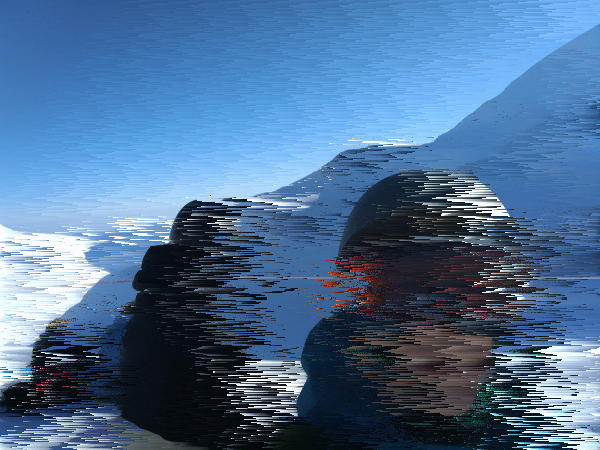
\includegraphics[width=\textwidth, height=\textheight, keepaspectratio]{example1.png}
%	\caption{Thats me. Source: {https://thecell.eu/}}
%	\label{fig:examplesOfImages}
%\end{figure}
%
%and even multiple images are possible
%
%\begin{figure}[H]
%	\centering
%	\subfigure{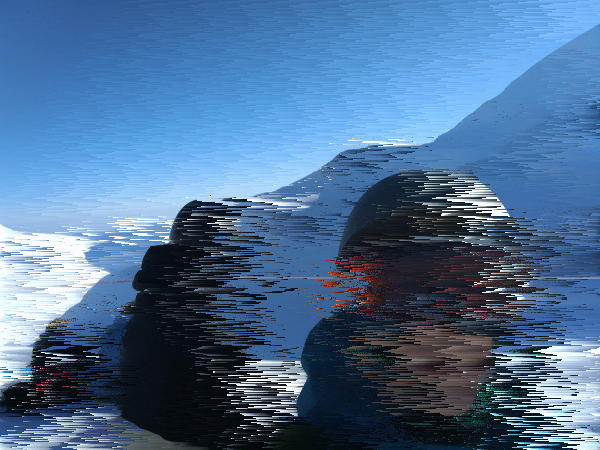
\includegraphics[width=0.4\textwidth]{example1.png}}
%	\subfigure{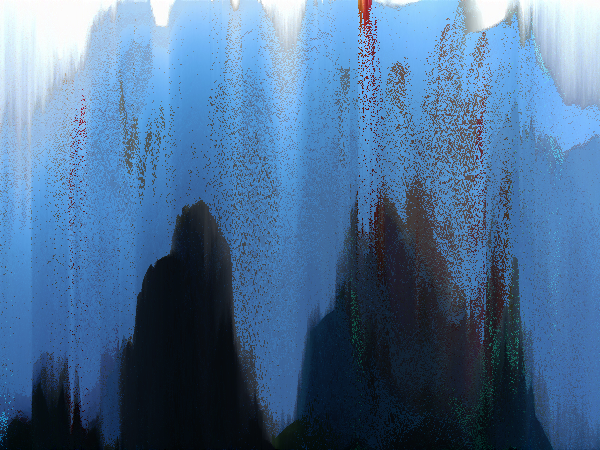
\includegraphics[width=0.4\textwidth]{example2.png}}
%	\subfigure{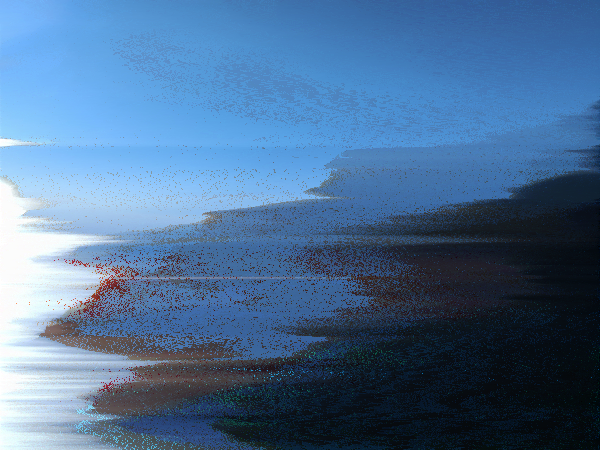
\includegraphics[width=1\textwidth]{example3.png}}
%	\caption{multiple images as an example}
%	\caption{if needed to reference separate it's possible like this}
%\end{figure}
%
%\subsection{Script code}
%A simple codeblock is possible take a look at this:
%\begin{lstlisting}
%<script>
%let aVar = "this is a JavaScript variable";
%console.log(aVar);
%</script>
%\end{lstlisting}
%
%\subsection{Tables etc.}
%\subsubsection{itemlist}
%\textbf{Lists} can be made as following:
%\begin{itemize}
%\item List an item once
%\item or twice
%\item just add more if needed
%\item sublists are possible aswell:
%\begin{itemize}
%\item List an item once \label{itm:ListAnItemOnce}
%\item or twice
%\item just add more if needed
%\end{itemize}
%\end{itemize}
%
%\subsubsection{more item examples}
%\begin{itemize}
%\item there are item lists
%\item like this one
%\end{itemize}
%\begin{enumerate}
%\item enumerations
%\item as seen here
%\end{enumerate}
%\begin{description}
%\item [Ant] and descriptions
%\item [Elephant] like these two
%\end{description}
%
%\subsubsection{Tables}
%If you are looking for tables, here it is:
%\begin{table}[H]
%\centering
%\begin{tabular}{ |c|c|c|c|c|c|c| }
%\hline
% & 1 & 2 & 3 & 4 & 5 & 6 \\
%\hline
%Dota 2 & 31 min & H & ++ & Z & $<$40\$ & Kosmetisch \\
%\hline
%PoE & $\infty$ & H & ++ & Z & $<$\$440 & Shoppunkte \\
%\hline
%The Witcher 3 & 48.5h & H \& C &  & Z & \$24 & AddOn \\
%\hline
%\end{tabular}
%\caption{Statistik Spiellänge wurde erfasst von \texttt{https://howlongtobeat.com} und \texttt{http://steamspy.com/.}}
%\label{table:1}
%\end{table}
%
%\subsection{math}
%\(
%\forall x \in X, \quad \exists y \leq \epsilon 
%\\
%\alpha, \beta, \gamma, \Gamma, \pi, \Pi, \phi, \varphi, \mu, \Phi
%\\
%\cos (2\theta) = \cos^2 \theta - \sin^2 \theta
%\\
%n^{22}
%\\
%\frac{n!}{k!(n-k)!} = \binom{n}{k}
%\\
%p = \frac{h}{2\pi i}\frac{\mathrm d}{\mathrm d x}\Psi
%\)
%
%\begin{multicols}{2}
%[
%\section{Multicolumns} All human things are subject to decay. And when fate summons, Monarchs must obey.
%]
%Hello, here is some text without a meaning.  This text should show what 
%a printed text will look like at this place.
%If you read this text, you will get no information.  Really?  Is there 
%no information?  Is there...
%More can be found here: \url{https://www.sharelatex.com/learn/Multiple_columns}
%\end{multicols}
%
%\section{some sections habe}
%\subsection{subsections}
%stahp
%\subsubsection{and even more subs}
%haha oh god.

\section{References and acronyms}

\printglossaries

%\renewcommand{\refname}{myBibliography}
\bibliography{myBibliography}
%\bibliographystyle{unsrtnat}
%\bibliographystyle{plainnat}
\bibliographystyle{unsrt}
%\bibliography{myBibliography}

%list the figures and tables in contents
%\addcontentsline{toc}{section}{\listfigurename}
%\addcontentsline{toc}{section}{\listtablename}

%print list
\listoffigures
\listoftables

%\nocite{*}

\end{document}